\chapter{ROCm 安裝指南}\label{AppendiceA}

在這個章節中,我們將介紹 ROCm 的安裝過程。安裝 ROCm 通常是使用 AMD GPU 的第一個步驟。因此,在開始開發或執行 GPU 程式之前,熟悉 ROCm 環境的安裝過程會有所幫助。

本章將介紹在 Ubuntu 20.04 LTS 作業系統上安裝 ROCm v5.4 的步驟。由於 ROCm 仍在積極開發,我們只會介紹所需的基本操作指令,並說明執行這些指令後的結果。隨著新版本的 ROCm 持續發布,本章部分內容可能會過時。因此,建議讀者在開始安裝之前,參考最新的安裝文件。ROCm 的安裝文件可在 \url{https://docs.amd.com} 取得。

\section{先備條件}

我們將示範如何在 Ubuntu 20.04 LTS 作業系統上安裝 ROCm。ROCm 可以支援多種不同的 Linux 作業系統發行版。目前 ROCm 並不支援 Microsoft Windows 作業系統,但 Windows 的支援可能會在近期推出。

ROCm 支援的作業系統如表格 \ref{table:rocm_supported_distros_and_kernel_versions} 所示。整體而言,ROCm 支援 Red Hat Enterprise Linux (RHEL)、SUSE Linux Enterprise Server (SLES) 和 Ubuntu 發行版。對於每個發行版,都有要求一個最低的核心版本(如 5.14, 4.18)。此外,系統上需要安裝一些額外的軟體套件,例如 \lstinline|wget|、\lstinline|gnupg2|、\lstinline|gawk| 和 \lstinline|curl|,因為這些是 ROCm 安裝腳本所需的必要工具。


\begin{table}[h!]
\centering
\caption{目前支援的 Linux 發行版與核心版本}
\label{table:rocm_supported_distros_and_kernel_versions}
\begin{tabular}{ll}
\hline
\textbf{作業系統} & \textbf{核心版本} \\ \hline  
RHEL 9.1 & 5.14 \\ 
RHEL 8.7 & 4.18 \\ 
RHEL 8.6 & 4.18 \\ 
SLES15 SP4 & 5.14.21 \\ 
Ubuntu 20.04.5 LTS & 5.15 \\ 
Ubuntu 22.04.1 LTS & 5.15, OEM 5.17 \\ \hline 
\end{tabular}
\end{table}


需要執行 GPU 程式的系統使用者必須加入適當的使用者群組。可以使用 groups 指令來檢查目前使用者所屬的群組。若要使用 GPU,使用者需加入 \lstinline|render| 或 \lstinline|video|(推薦)群組之一。可以使用指令 \lstinline|sudo usermod -a -G [群組名稱] [使用者名稱]| 來將使用者加入特定的群組。

在購買 GPU 硬體之前,應確認預計要購買的 GPU 是否被 ROCm 平台所之援(請參閱表格 \ref{table:rocm_supported_gpus})。

\begin{table}[h!]
\centering
\caption{ROCm 支援的 GPU 型號}
\label{table:rocm_supported_gpus}
\begin{tabular}{lll}
\hline
\textbf{GPU 系列} & \textbf{GPU} & \textbf{GFX ID} \\ \hline
\multirow{4}{*}{GCN} & AMD Radeon Instinct\texttrademark\ MI50 & \multirow{4}{*}{GFX906} \\ 
 & AMD Radeon Instinct\texttrademark\ MI60 & \\ 
 & AMD Radeon\texttrademark\ VII &  \\ 
 & AMD Radeon\texttrademark\ Pro VII &  \\ 
\multirow{2}{*}{RDNA} & AMD Radeon\texttrademark\ Pro W6800 & \multirow{2}{*}{GFX1030} \\ 
 & AMD Radeon\texttrademark\ Pro V620 &  \\ 
\multirow{2}{*}{CDNA} & AMD Instinct\texttrademark\ MI100 & GFX908 \\ 
 & AMD Instinct\texttrademark\ MI200 & GFX90a \\ \hline
\end{tabular}
\end{table}

\section{理解 ROCm 套件}

ROCm 是一個包含許多軟體套件的複雜生態系統。完整的套件列表可以參見圖 \ref{fig:rocm_packages}。這些套件可能有複雜的依賴性關係。為了避免使用者需要逐一安裝套件,ROCm 將這些套件分組為元套件 (meta-package)(完整列表請參見表格 \ref{table:rocm_meta_packages})。使用者通常會選擇安裝元套件,而非獨立安裝各個套件。

\begin{figure}
    \centering
    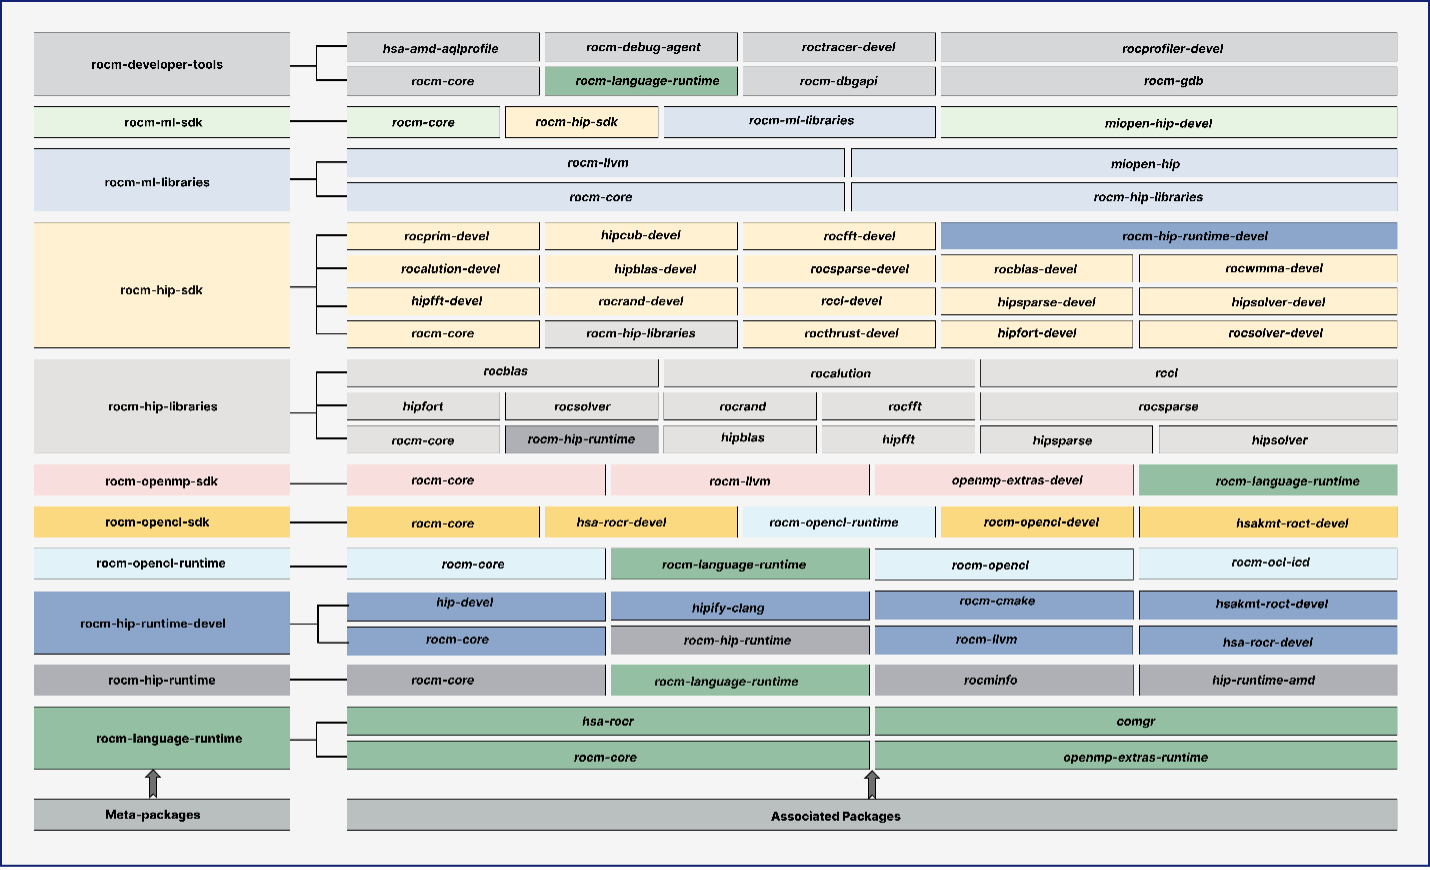
\includegraphics[width=1\linewidth]{Appendici/MetaPackages.png}
    \caption{ROCm 元套件的列表以及包含在元套件中的各個獨立套件}
    \label{fig:rocm_packages}
\end{figure}


\section{安裝}

在此概論中,我們介紹兩種安裝 ROCm 的方法,包含安裝程式腳本的方法與套件管理器的方法。

\subsection{安裝程式腳本方法}
\label{sec:rocm_installer_method}
安裝程式腳本方法自動化了 AMDGPU 和 ROCm 的安裝過程。安裝程式腳本會處理 ROCm 的完整安裝過程,包括設定儲存庫、清理檔案系統、更新和安裝所需的驅動程式與元套件。使用此方法,系統對 ROCm 安裝過程有更多控制權。因此,那些對標準 Linux 指令不太熟悉的使用者可以選擇此方法來安裝 ROCm。可以使用以下指令下載並安裝安裝程式:

\begin{lstlisting}[caption={使用安裝程式腳本安裝 ROCm 所需指令}, label={lst:a1}]
sudo apt-get update
wget https://repo.radeon.com/amdgpu-install/5.4.3/ubuntu/focal/amdgpu-install_5.4.50403-1_all.deb
sudo apt-get install ./amdgpu-install_5.4.50403-1_all.deb
\end{lstlisting}

上述指令應該會安裝一個可以幫助管理 ROCm 套件的 \lstinline|amdgpu-install| 程式。如要安裝 ROCm,我們可以使用 \lstinline|sudo ./amdgpu-install| 指令執行安裝。此外,使用者也可以透過像是 \lstinline|sudo amdgpu-install --usecase=rocm| 的指令來安裝特定的使用案例。如果使用者希望一次安裝多個使用案例,可以在 \lstinline|usecase| 參數中指定多個值,並以逗號分隔。例如,指令 \lstinline|sudo amdgpu-install --usecase=rocm,hiplibsdk| 會同時安裝 ROCm 和 \lstinline|hiplibsdk| 兩個使用案例。使用 \lstinline|sudo amdgpu-install --list-usecase| 可以顯示所有可用的使用案例的列表。


\subsection{套件管理器方法}

套件管理器方法提供使用者更多安裝選項的靈活性,但在安裝過程中需要更多的使用者操作。建議此方法僅供進階使用者使用。總體來說,使用套件管理器安裝 ROCm 包括以下六個步驟:

\paragraph{步驟 1:安裝 Linux 核心標頭與開發套件}
使用套件管理器方法的前置步驟之一是安裝正確的 Linux 核心標頭與開發套件。

可以使用指令 \lstinline!sudo dpkg -l | grep linux-headers! 來檢查已安裝的核心標頭版本。例如,輸出的結果可能是 \lstinline|ii linux-headers-5.15.0-41-generic 5.15.0-41.44 20.04.1 amd64 Linux kernel headers for version 5.15.0 on 64 bit x86 SMP|。
類似地,可以使用指令 \lstinline!sudo dpkg -l | grep linux-modules-extra! 來列出開發套件,在作者的系統中輸出的結果為
\lstinline|ii linux-modules-extra-5.15.0-41-generic 5.15.0-41.44 20.04.1 amd64 Linux kernel extra modules for version 5.15.0 on 64 bit x86 SMP|。
如果當前版本的 Linux 標頭不符合表 \ref{table:rocm_supported_distros_and_kernel_versions} 中列出的要求,使用者需要使用指令 \lstinline|sudo apt install linux-headers-$(uname -r) linux-modules-extra-$(uname -r)| 來安裝所需的 Linux 標頭。


\paragraph{步驟 2:安裝 AMD GPU 驅動程式}
接下來,我們會使用套件管理器安裝 AMD GPU 驅動程式。套件管理器要求套件必須加密,因此需要安裝一組 GNU Privacy Guard(GPG)金鑰。安裝 GPG 金鑰的指令為:

\lstinline!curl -fsSL https://repo.radeon.com/rocm/rocm.gpg.key | sudo gpg --dearmor -o /etc/apt/trusted.gpg.d/rocm-keyring.gpg!。

接下來,使用以下指令將 AMD GPU 儲存庫新增到 Ubuntu 的套件管理器中:

\lstinline!echo 'deb [arch=amd64 signed-by=/etc/apt/trusted.gpg.d/rocm-keyring.gpg] https://repo.radeon.com/amdgpu/5.4.3/ubuntu focal main' | sudo tee /etc/apt/sources.list.d/amdgpu.list!。
新增儲存庫後,別忘了執行 \lstinline|sudo apt-get update|,讓套件管理器能夠取得套件資訊。
最後,使用 \lstinline|sudo apt install amdgpu-dkms| 來安裝 AMD GPU 驅動程式。安裝完成後,需要重新啟動系統。

\paragraph{步驟 3:安裝 ROCm 環境}
為了安裝 ROCm 環境,我們需要使用以下指令將外部資源加入到 Ubuntu 的套件管理器中:

\lstinline!echo 'deb [arch=amd64 signed-by=/etc/apt/trusted.gpg.d/rocm-keyring.gpg] https://repo.radeon.com/rocm/apt/5.4.3 focal main' | sudo tee /etc/apt/sources.list.d/rocm.list!

此指令會建立 \lstinline|rocm.list|,其中包含提供套件的 URL。

接下來,我們需要透過以下指令修改優先權:

\lstinline!echo -e 'Package: *\nPin: release o=repo.radeon.com\nPin-Priority: 600' | sudo tee /etc/apt/preferences.d/rocm-pin-600! 

透過為 ROCm 套件設定較高的優先權,我們可以在更新套件時保持穩定版本的 Ubuntu。在新增套件來源並修改優先設定後,我們仍然需要執行 \lstinline|sudo apt-get update|。


\subsection{驗證安裝}
無論使用哪種安裝方法,我們都需要驗證安裝是否成功。如果執行過程中出現錯誤,使用者應該首先檢查 ROCm 安裝是否已損壞。

首先,我們可以檢查 \lstinline|/opt/rocm|目錄是否包含預期的執行檔,例如 \lstinline|rocm-smi|,以及 ROCm 函式庫,例如 \lstinline|librocblas.so|。
其次,我們可以檢查驅動程式是否正常運作。可以使用 \lstinline|dkms status| 指令檢查目前正在使用的驅動程式。例如,在作者的系統中,執行此指令會顯示輸出:\lstinline|amdgpu, 5.16.9.22.20-1438746~20.04, 5.4.0-121-generic, x86_64: installed|。這表示驅動程式已正確安裝並正在使用。

再來,我們應該檢查是否有程式能夠偵測到 GPU 硬體並取得 GPU 的屬性。我們可以執行 \lstinline|/opt/rocm/bin/rocminfo| 或 \lstinline|/opt/rocm/opencl/bin/clinfo| 來取得硬體屬性。如果這兩個程式能夠順利執行並且顯示系統中安裝的 GPU,則表示 ROCm 環境已正確安裝並且正常運作。

最後,我們可以使用平常的 Ubuntu 套件安裝指令來安裝元套件。指令為 \lstinline|sudo apt install <套件名稱>|。例如,如果我們想安裝最常使用的 ROCm 功能,可以使用 \lstinline|sudo apt install rocm|。


\section{更新 ROCm}
保持新版本的 ROCm 非常重要,因為工具和函式庫會不斷收到新的功能更新、錯誤修復、效能改善和安全性更新。和安裝過程類似,使用者可以選擇使用安裝程式或是 Linux 發行版提供的套件管理器。

若要使用安裝程式腳本方法,首先需要按照章節 \ref{sec:rocm_installer_method} 所描述的步驟安裝安裝程式。接下來,升級套件版本的過程與全新安裝相同。若要更新特定的使用案例,可以使用指令 \lstinline|sudo amdgpu-install --usecase=<使用案例>|。

若是使用套件管理器更新 ROCm,則會需要較多指令。首先,我們需要更新 AMD GPU 驅動程式套件的外部來源,使用以下指令:

\lstinline!echo 'deb [arch=amd64 signed-by=/etc/apt/trusted.gpg.d/rocm-keyring.gpg] <amdgpu baseurl> focal main' | sudo tee /etc/apt/sources.list.d/amdgpu.list!

修改來源清單後需要執行 \lstinline|sudo apt-get update|。接著,我們可以使用指令 \lstinline|sudo apt install amdgpu-dkms| 來更新驅動程式。同樣,安裝完成後,需要重新啟動系統。

最後,我們需要對 ROCm 套件重複此過程。使用以下指令來修改外部來源:

\lstinline!echo 'deb [arch=amd64 signed-by=/etc/apt/trusted.gpg.d/rocm-keyring.gpg] <rocm baseurl> focal main' | sudo tee /etc/apt/sources.list.d/rocm.list!

\lstinline!echo -e 'Package: *\nPin: release o=repo.radeon.com\nPin-Priority: 600' | sudo tee /etc/apt/preferences.d/rocm-pin-600!

接著,我們可以使用套件管理器更新 ROCm 套件,指令為:\lstinline|sudo apt install --only-upgrade <套件名稱>|。

\section{解除安裝 ROCm}
若要解除安裝 ROCm,我們可以選擇使用安裝程式腳本(在這種情況下是解除安裝程式)或是 Linux 發行版的套件管理器。如果 ROCm 是透過安裝程式腳本安裝的,解除安裝程式會與安裝程式一併提供。解除安裝 ROCm 只需執行 \lstinline|sudo amdgpu-uninstall| 即可。
Ubuntu 的套件管理器可以輕鬆解除安裝 ROCm 或特定的使用案例。指令為:
\lstinline|sudo apt autoremove <套件名稱>|。


\begin{table}[h!]
\centering
\caption{ROCm 的元套件}
\label{table:rocm_meta_packages}
\begin{tabular}{lp{0.6\linewidth}}
\hline
\textbf{元套件}               & \textbf{說明}  \\
\hline
\lstinline|rocm-hip-libraries|            & \lstinline|rocm-hip-libraries| 會安裝為 AMD 平台優化的 HIP 函式庫。                                            \\
\lstinline|rocm-hip-runtime|              & \lstinline|rocm-hip-runtime| 會安裝運行在 AMD 平台上以 HIP 撰寫的應用程式所需的套件            \\
\lstinline|rocm-hip-runtime-devel|        & \lstinline|rocm-hip-runtime-devel| 會安裝開發基於 HIP 的應用程式或將其從 CUDA 移植過來所需的套件   \\
\lstinline|rocm-hip-sdk|                  & \lstinline|rocm-hip-sdk| 會安裝開發/移植使用 HIP 的應用程式所需的套件以及為 AMD 平台提供的函式庫  \\
\lstinline|rocm-language-runtime|         & \lstinline|rocm-language-runtime| 會安裝 ROCm 執行環境   \\
\lstinline|rocm-ml-libraries|             & \lstinline|rocm-ml-libraries| 會安裝關鍵的機器學習函式庫套件(主要是 MIOpen)  \\
\lstinline|rocm-ml-sdk|                   & \lstinline|rocm-ml-sdk| 會安裝開發和運行使用為 AMD 平台優化的機器學習運算單元的應用程式所需的套件  \\
\lstinline|rocm-opencl-runtime|           & \lstinline|rocm-opencl-runtime| 會安裝在 AMD 平台上執行基於 OpenCL 的應用程式所需的套件   \\
\lstinline|rocm-opencl-sdk|               & \lstinline|rocm-opencl-sdk| 會安裝在 AMD 平台上開發基於 OpenCL 的應用程式所需的套件  \\
\lstinline|rocm-openmp-runtime|           & \lstinline|rocm-openmp-runtime| 會安裝在 AMD 平台上執行基於 OpenMP 的應用程式所需的套件  \\
\lstinline|rocm-openmp-sdk|               & \lstinline|rocm-openmp-sdk| 會安裝在 AMD 平台上開發基於 OpenMP 的應用程式所需的套件   \\
\hline
\end{tabular}
\end{table}
